% ==========================================================================
% INFO 4617 Web Data Science -- Week 1: Introduction & Setup (Chapter 1)
% Build:  latexmk -pdf week-01.tex   (from this folder; no env vars needed)
% (or run `make` from the slides/ directory to build every deck)
%
% NOTE: The semester starts Thursday, Aug 20, so this week meets FRIDAY ONLY.
% This is a single-session intro deck, not the usual Mon/Wed/Fri shape.
%
% Environment setup (Anaconda, first request) is NOT in this deck -- it moved
% to handouts/setup.md so class time protects the textbook-revision activity.
% ==========================================================================
\documentclass[9pt,aspectratio=169]{beamer}
% Resolve the shared theme/preamble in ../common/ when compiling this
% file directly from its own folder (no TEXINPUTS needed).
\makeatletter\def\input@path{{../common/}}\makeatother
% ==========================================================================
% Shared preamble for INFO 4617 Web Data Science weekly lecture decks
% Based on the Gotham beamer theme (vendored in this directory).
% Each week's slides.tex does:  % ==========================================================================
% Shared preamble for INFO 4617 Web Data Science weekly lecture decks
% Based on the Gotham beamer theme (vendored in this directory).
% Each week's slides.tex does:  % ==========================================================================
% Shared preamble for INFO 4617 Web Data Science weekly lecture decks
% Based on the Gotham beamer theme (vendored in this directory).
% Each week's slides.tex does:  \input{preamble}  (with common/ on TEXINPUTS)
% then sets \title/\subtitle/\author/\date and \begin{document}.
% ==========================================================================

\usetheme{gotham}

\usepackage{fbb}
\usepackage{booktabs}
\usepackage{graphicx}
\usepackage{tikz}
\usepackage{xcolor}
\usepackage{multirow}
\usepackage{listings}
\usetikzlibrary{positioning, arrows.meta, shapes}

% Bibliography
\usepackage[style=authoryear,
            backend=biber,
            maxcitenames=1,
            uniquename=false,
            uniquelist=false]{biblatex}
\addbibresource{bibliography.bib}

\gothamset{sectiontocframe default=off}

% ------------------------------------------------------------------ colors
\definecolor{cugold}{HTML}{CFB87C}
\definecolor{tab-red}{HTML}{E15759}
\definecolor{tab-orange}{HTML}{F28E2B}
\definecolor{tab-blue}{HTML}{4E79A7}
\definecolor{tab-cyan}{HTML}{76B7B2}
\definecolor{tab-green}{HTML}{59A14F}
\definecolor{tab-yellow}{HTML}{EDC948}
\definecolor{tab-purple}{HTML}{B07AA1}
\definecolor{tab-pink}{HTML}{FF9DA7}
\definecolor{tab-brown}{HTML}{9C755F}
\definecolor{tab-gray}{HTML}{BAB0AC}

\setbeamercolor{frametitle}{fg=black, bg=cugold}
\setbeamercolor{progress bar}{fg=cugold, bg=cugold!20}

\setbeamercolor{block title alerted}{fg=black, bg=cugold}
\setbeamercolor{block body alerted}{fg=black, bg=cugold!10}

% ------------------------------------------------------------------ footline
\setbeamertemplate{footline}{
  \begin{beamercolorbox}[wd=\paperwidth,ht=2.5ex,dp=1ex,right]{footline}
    {\footnotesize \insertframenumber{} of \inserttotalframenumber}
    \hspace*{2ex}
  \end{beamercolorbox}
}

% ------------------------------------------------------------------ helpers
\newcommand{\bottomcite}[1]{
    \vspace*{\fill}
    \vspace{-\baselineskip}
    {\tiny
    \rule{\textwidth}{0.3pt}\\
    #1
    }
    \vspace{0.5ex}
}

% Consistent code styling for the Wednesday "applied notebook" frames.
\lstdefinestyle{wds}{
    basicstyle=\ttfamily\scriptsize,
    keywordstyle=\color{tab-blue}\bfseries,
    commentstyle=\color{tab-green},
    stringstyle=\color{tab-orange},
    showstringspaces=false,
    breaklines=true,
    columns=fullflexible,
    language=Python,
    aboveskip=0.4em,
    belowskip=0.4em,
}
\lstset{style=wds}

% \dayband{Day}{Topic} -- a lightweight section divider label used to mark
% Monday / Wednesday / Friday within a week's deck.
\newcommand{\dayband}[2]{{\large\textbf{#1}}\;\textcolor{tab-gray}{\textbar}\;#2}
  (with common/ on TEXINPUTS)
% then sets \title/\subtitle/\author/\date and \begin{document}.
% ==========================================================================

\usetheme{gotham}

\usepackage{fbb}
\usepackage{booktabs}
\usepackage{graphicx}
\usepackage{tikz}
\usepackage{xcolor}
\usepackage{multirow}
\usepackage{listings}
\usetikzlibrary{positioning, arrows.meta, shapes}

% Bibliography
\usepackage[style=authoryear,
            backend=biber,
            maxcitenames=1,
            uniquename=false,
            uniquelist=false]{biblatex}
\addbibresource{bibliography.bib}

\gothamset{sectiontocframe default=off}

% ------------------------------------------------------------------ colors
\definecolor{cugold}{HTML}{CFB87C}
\definecolor{tab-red}{HTML}{E15759}
\definecolor{tab-orange}{HTML}{F28E2B}
\definecolor{tab-blue}{HTML}{4E79A7}
\definecolor{tab-cyan}{HTML}{76B7B2}
\definecolor{tab-green}{HTML}{59A14F}
\definecolor{tab-yellow}{HTML}{EDC948}
\definecolor{tab-purple}{HTML}{B07AA1}
\definecolor{tab-pink}{HTML}{FF9DA7}
\definecolor{tab-brown}{HTML}{9C755F}
\definecolor{tab-gray}{HTML}{BAB0AC}

\setbeamercolor{frametitle}{fg=black, bg=cugold}
\setbeamercolor{progress bar}{fg=cugold, bg=cugold!20}

\setbeamercolor{block title alerted}{fg=black, bg=cugold}
\setbeamercolor{block body alerted}{fg=black, bg=cugold!10}

% ------------------------------------------------------------------ footline
\setbeamertemplate{footline}{
  \begin{beamercolorbox}[wd=\paperwidth,ht=2.5ex,dp=1ex,right]{footline}
    {\footnotesize \insertframenumber{} of \inserttotalframenumber}
    \hspace*{2ex}
  \end{beamercolorbox}
}

% ------------------------------------------------------------------ helpers
\newcommand{\bottomcite}[1]{
    \vspace*{\fill}
    \vspace{-\baselineskip}
    {\tiny
    \rule{\textwidth}{0.3pt}\\
    #1
    }
    \vspace{0.5ex}
}

% Consistent code styling for the Wednesday "applied notebook" frames.
\lstdefinestyle{wds}{
    basicstyle=\ttfamily\scriptsize,
    keywordstyle=\color{tab-blue}\bfseries,
    commentstyle=\color{tab-green},
    stringstyle=\color{tab-orange},
    showstringspaces=false,
    breaklines=true,
    columns=fullflexible,
    language=Python,
    aboveskip=0.4em,
    belowskip=0.4em,
}
\lstset{style=wds}

% \dayband{Day}{Topic} -- a lightweight section divider label used to mark
% Monday / Wednesday / Friday within a week's deck.
\newcommand{\dayband}[2]{{\large\textbf{#1}}\;\textcolor{tab-gray}{\textbar}\;#2}
  (with common/ on TEXINPUTS)
% then sets \title/\subtitle/\author/\date and \begin{document}.
% ==========================================================================

\usetheme{gotham}

\usepackage{fbb}
\usepackage{booktabs}
\usepackage{graphicx}
\usepackage{tikz}
\usepackage{xcolor}
\usepackage{multirow}
\usepackage{listings}
\usetikzlibrary{positioning, arrows.meta, shapes}

% Bibliography
\usepackage[style=authoryear,
            backend=biber,
            maxcitenames=1,
            uniquename=false,
            uniquelist=false]{biblatex}
\addbibresource{bibliography.bib}

\gothamset{sectiontocframe default=off}

% ------------------------------------------------------------------ colors
\definecolor{cugold}{HTML}{CFB87C}
\definecolor{tab-red}{HTML}{E15759}
\definecolor{tab-orange}{HTML}{F28E2B}
\definecolor{tab-blue}{HTML}{4E79A7}
\definecolor{tab-cyan}{HTML}{76B7B2}
\definecolor{tab-green}{HTML}{59A14F}
\definecolor{tab-yellow}{HTML}{EDC948}
\definecolor{tab-purple}{HTML}{B07AA1}
\definecolor{tab-pink}{HTML}{FF9DA7}
\definecolor{tab-brown}{HTML}{9C755F}
\definecolor{tab-gray}{HTML}{BAB0AC}

\setbeamercolor{frametitle}{fg=black, bg=cugold}
\setbeamercolor{progress bar}{fg=cugold, bg=cugold!20}

\setbeamercolor{block title alerted}{fg=black, bg=cugold}
\setbeamercolor{block body alerted}{fg=black, bg=cugold!10}

% ------------------------------------------------------------------ footline
\setbeamertemplate{footline}{
  \begin{beamercolorbox}[wd=\paperwidth,ht=2.5ex,dp=1ex,right]{footline}
    {\footnotesize \insertframenumber{} of \inserttotalframenumber}
    \hspace*{2ex}
  \end{beamercolorbox}
}

% ------------------------------------------------------------------ helpers
\newcommand{\bottomcite}[1]{
    \vspace*{\fill}
    \vspace{-\baselineskip}
    {\tiny
    \rule{\textwidth}{0.3pt}\\
    #1
    }
    \vspace{0.5ex}
}

% Consistent code styling for the Wednesday "applied notebook" frames.
\lstdefinestyle{wds}{
    basicstyle=\ttfamily\scriptsize,
    keywordstyle=\color{tab-blue}\bfseries,
    commentstyle=\color{tab-green},
    stringstyle=\color{tab-orange},
    showstringspaces=false,
    breaklines=true,
    columns=fullflexible,
    language=Python,
    aboveskip=0.4em,
    belowskip=0.4em,
}
\lstset{style=wds}

% \dayband{Day}{Topic} -- a lightweight section divider label used to mark
% Monday / Wednesday / Friday within a week's deck.
\newcommand{\dayband}[2]{{\large\textbf{#1}}\;\textcolor{tab-gray}{\textbar}\;#2}


\title[Week 1 · Introduction]{{\Huge Introduction \& Setup}}
\subtitle{Week 1 · Foundations module · Textbook Chapter 1}
\author[Keegan]{\textbf{Brian C. Keegan, Ph.D.} \\ Associate Professor, Department of Information Science \\ University of Colorado Boulder}
\date{Friday, August 21, 2026}

\begin{document}

\maketitle

% -------------------------------------------------------------------------
\begin{frame}{This week at a glance}
    \begin{columns}[T]
        \begin{column}{0.6\textwidth}
            Welcome to Web Data Science. The semester starts Thursday, so this week we meet \textbf{Friday only}

            \bigskip
            Today is orientation and introduction to GitHub.

            \bigskip

            \dayband{Friday}{Orientation, the book \& setting up GitHub}
            \begin{itemize}\small
                \item What web data science is and why it matters
                \item How the class works and how you're graded
                \item Our unusual textbook
                \item Git \& GitHub
            \end{itemize}

            \bigskip

            The \textbf{Monday $\rightarrow$ Wednesday $\rightarrow$ Friday} rhythm begins next week.
        \end{column}
        \begin{column}{0.35\textwidth}
            \begin{block}{Our textbook}
                \footnotesize \url{https://cuinfoscience.github.io/Web-Data-Science-Book/}
            \end{block}
            \begin{block}{Its source code}
                \footnotesize \url{https://github.com/cuinfoscience/Web-Data-Science-Book}
            \end{block}
            \begin{alertblock}{Before Monday}
                \footnotesize Work through \texttt{handouts/setup.md}: Anaconda, Git, and a \textbf{free} GitHub account. Bring a laptop --- today included.
            \end{alertblock}
        \end{column}
    \end{columns}
\end{frame}

% =========================================================================
\section{Welcome}
% =========================================================================

\begin{frame}{Meet your instructor}
    \begin{columns}[T]
        \begin{column}{0.6\textwidth}
            \textbf{Brian C. Keegan} --- Associate Professor
            \begin{itemize}\small
                \item Born in Medford, Oregon
                \item Grew up outside Las Vegas, Nevada
                \item Mechanical Engineering and Science, Technology \& Society, MIT, 2002--06
                \item Bartender and \href{https://infinite.mit.edu/collection/mit-150-interviews/}{oral historian}
                \item Ph.D.\ in Media, Technology \& Society, Northwestern, 2007--2012
                \item Postdoc in computational social science, Northeastern, 2012--14
                \item Data scientist, Harvard Business School, 2014--16
                \item CU Boulder Information Science, 2016--present
                \item Visiting scientist, Harvard Population Center, 2025--26
            \end{itemize}
            \medskip
            \url{brianckeegan.com}
        \end{column}
        \begin{column}{0.35\textwidth}
            \begin{block}{What I study}
                \footnotesize
                \begin{itemize}\footnotesize
                    \item High-tempo online collaborations
                    \item Public interest data science
                    \item Platform governance and migration
                \end{itemize}
            \end{block}
        \end{column}
    \end{columns}
\end{frame}

\begin{frame}{What is web data science?}
    \begin{columns}[T]
        \begin{column}{0.6\textwidth}
            The World Wide Web is the largest, most dynamic, and most contested data source ever created

            \bigskip
            The web is a data source and web data science is how you get, clean, and use it

            \bigskip
            \textbf{Web data science} is the practice of retrieving data from the web, parsing it into structured formats, and analyzing it to produce knowledge.
        \end{column}
        \begin{column}{0.35\textwidth}
            \begin{block}{Not your usual dataset}
                \footnotesize The web is \textbf{not a database}. Data arrives as:
                \begin{itemize}\footnotesize
                    \item HTML tables buried slopified websites
                    \item JSON from rate-limited APIs
                    \item scanned PDFs from a FOIA request
                    \item pages that might vanish tomorrow
                \end{itemize}
            \end{block}
        \end{column}
    \end{columns}
\end{frame}

\begin{frame}{Data in the public interest}
    \begin{columns}[T]
        \begin{column}{0.6\textwidth}
            Many disciplines and professions have developed their own local dialects of web data science: computational social science, data journalism, and civic technology

            \bigskip
            Data is power and that power that should serve the public.

            \bigskip
            Who gets to access and benefit from web data is an extremely live issue right now: surveillance, AI, copyright
            
        \end{column}
        \begin{column}{0.35\textwidth}
            \begin{alertblock}{Classic readings}

            \begin{center}
                
\includegraphics[width=.5\textwidth]{../common/cupids-logo.png}
            \end{center}
            \begin{block}{Ask me about CUPIDS Lab}
                \url{https://www.cupids-lab.org/}
            \end{block}
            \end{alertblock}
        \end{column}
    \end{columns}
\end{frame}

\begin{frame}{Common sequence across topics}
    \begin{columns}[T]
        \begin{column}{0.6\textwidth}
            Every week in this course follows a common sequence:

            \bigskip

            \begin{center}
                {\large \textbf{retrieve $\rightarrow$ parse $\rightarrow$ analyze}}
            \end{center}
            

            \bigskip

            \begin{itemize}
                \item \textbf{Retrieve} an HTML, JSON, or PDF file with \texttt{requests}
                \item \textbf{Parse} it into data: JSON, CSV, \textit{etc}.
                \item Load into a \textbf{pandas} DataFrame
                \item \textbf{Analyze} or visualize the result
            \end{itemize}

            \bigskip
            You can collect the data and make this visualization after reading the Ch.~01 of the textbook, ``Your First Request.''
        \end{column}
        \begin{column}{0.35\textwidth}
            \centering
            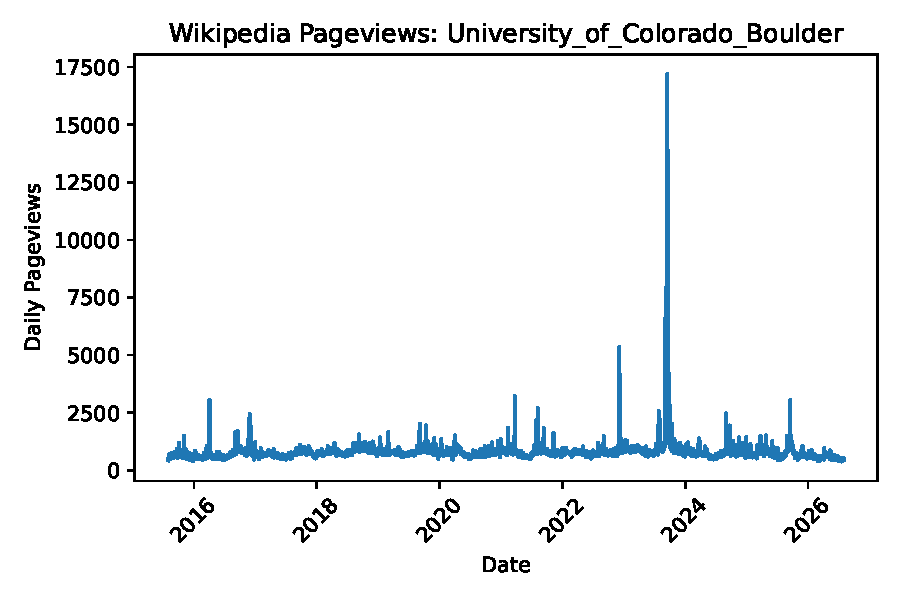
\includegraphics[width=\textwidth]{img/pageviews.pdf}
        \end{column}
    \end{columns}
\end{frame}

\begin{frame}{The data science mindset}
    Technical fluency is not enough. Four dispositions will serve you all semester:
    \begin{itemize}
        \item \textcolor{tab-green}{\textbf{Growth mindset}} --- ability develops through effort. Treat each error as a learning signal, not evidence of inadequacy.
        \item \textcolor{tab-blue}{\textbf{Computational thinking}} --- decompose, recognize patterns, abstract, and specify unambiguous steps.
        \item \textcolor{tab-orange}{\textbf{The hacker ethic}} --- sharing, openness, curiosity, and a bias toward action. The libraries we will use exist because people shared their work.
        \item \textcolor{tab-purple}{\textbf{Scientific norms}} --- communalism, skepticism, and reproducibility. Document your methods; question yours and others' data; report limitations.
    \end{itemize}
\end{frame}

% =========================================================================
\section{How this class works}
% =========================================================================

\begin{frame}{The weekly rhythm}
    \begin{columns}[T]
        \begin{column}{0.6\textwidth}
            Starting next week, every week runs on the same three-beat rhythm:

            \bigskip

            \dayband{Monday}{Concept + notebook intro}
            \begin{itemize}\small
                \item Lecture --- Introduce the week's ideas and the companion notebook, you read the week's textbook chapter
            \end{itemize}
            \medskip
            \dayband{Wednesday}{Notebook lab}
            \begin{itemize}\small
                \item Hands-on --- we work and debug the chapter's code together, live
            \end{itemize}
            \medskip
            \dayband{Friday}{Textbook revisions}
            \begin{itemize}\small
                \item Fix --- submit issues and propose pull requests that improve the textbook and notebooks
            \end{itemize}
        \end{column}
        \begin{column}{0.35\textwidth}
            \centering
            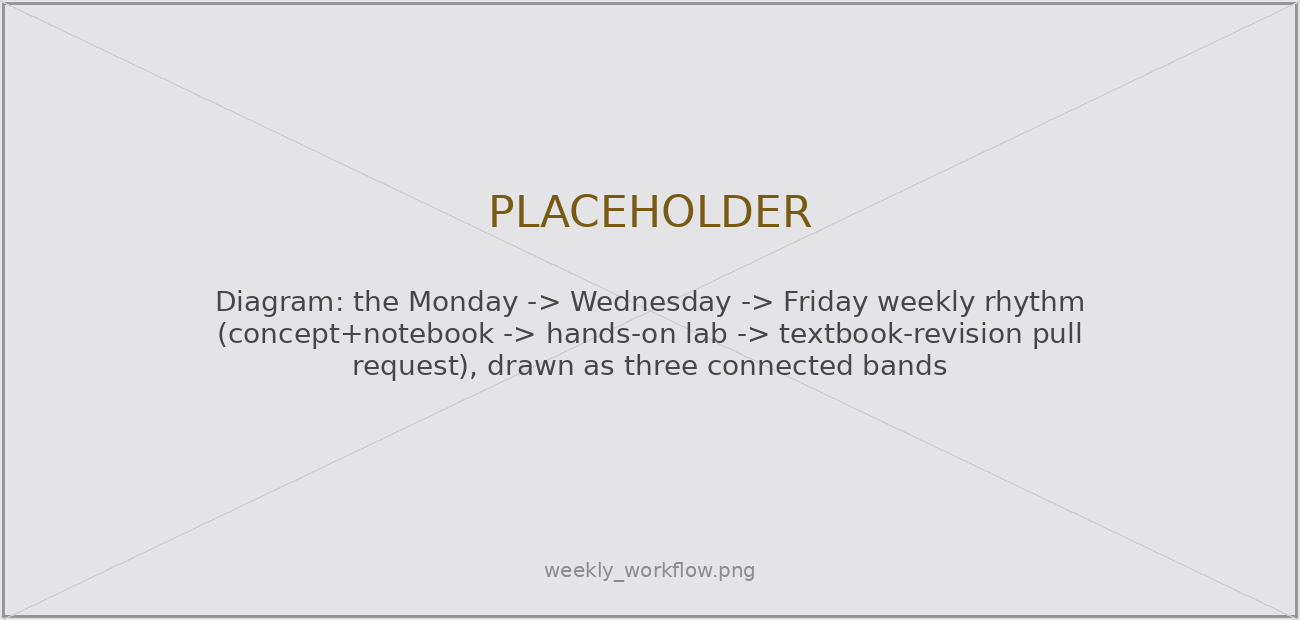
\includegraphics[width=\textwidth]{img/weekly_workflow.png}\\
            {\scriptsize Concept, then practice, then contribution.}
        \end{column}
    \end{columns}
    \bottomcite{This week is the exception --- Friday only. The full rhythm begins next week.}
\end{frame}

\begin{frame}{How you're evaluated}
    \begin{columns}[T]
        \begin{column}{0.6\textwidth}
            Your grade is \textbf{what you build}, not what you memorize:
            \medskip
            \begin{itemize}
                \item \textcolor{tab-blue}{\textbf{Notebook Labs --- 30\%}}\\ {\small weekly, hands-on data-collection work}
                \item \textcolor{tab-green}{\textbf{Textbook Revisions --- 15\%}}\\ {\small pull requests + peer reviews that improve the book}
                \item \textcolor{tab-orange}{\textbf{Attendance --- 15\%}}\\ {\small showing up, participating, daily notes}
                \item \textcolor{tab-purple}{\textbf{Final Project --- 40\%}}\\ {\small a research design + real data collection + analysis}
            \end{itemize}
        \end{column}
        \begin{column}{0.35\textwidth}
            \begin{block}{No exams}
                \footnotesize No midterm and no final. You demonstrate learning by \textbf{doing the work of a web data scientist} by collecting data, contributing to a shared resource, and building your own project.
            \end{block}
        \end{column}
    \end{columns}
\end{frame}

\begin{frame}{Course outline}
\begin{table}[ht]
\footnotesize
\centering
    \begin{tabular}{cccc}
        \toprule[.15em]
        \textbf{Module} & \textbf{Week} & \textbf{Dates} & \textbf{Topics} \\
        \cmidrule[.1em](lr){1-4}

        \multirow{5}{*}[0pt]{\textit{Foundations}}
            & 1 & Aug.~21 & Introduction \& setup \\
            & 2 & Aug.~24--28 & Ethics, law \& responsible collection \\
            & 3 & Aug.~31--Sep.~4 & The post-API age \\
            & 4 & Sep.~9--11 & Data formats: XML \& JSON \\
            & 5 & Sep.~14--18 & Web architecture \& protocols \\ \cmidrule[.1em](lr){1-4}

        \multirow{4}{*}[0pt]{\textit{Documents}}
            & 6 & Sep.~21--25 & Parsing static web pages \\
            & 7 & Sep.~28--Oct.~2 & Archived web pages \\
            & 8 & Oct.~5--9 & Dynamic web pages with Selenium \\
            & 9 & Oct.~12--16 & Extracting data from PDFs \\ \cmidrule[.1em](lr){1-4}

        \multirow{4}{*}[0pt]{\textit{APIs}}
            & 10 & Oct.~19--23 & Wikipedia APIs \\
            & 11 & Oct.~26--30 & Government data APIs \\
            & 12 & Nov.~2--6 & Social \& media platform APIs \\
            & 13 & Nov.~9--13 & AI \& language-model APIs \\ \cmidrule[.1em](lr){1-4}

        \multirow{3}{*}[0pt]{\textit{Practice}}
            & 14 & Nov.~16--20 & Automating data collection \\
            & 15 & Nov.~23--27 & \textbf{No class: Fall Break} \\
            & 16 & Nov.~30--Dec.~4 & Research design \& final presentations \\
            \cmidrule[.1em](lr){1-4}
            & \multicolumn{3}{c}{\textbf{Final Project due Friday, December 11}} \\

        \bottomrule[.15em]
    \end{tabular}
\end{table}
    
\end{frame}

\begin{frame}{Documentation and testing}
    \begin{columns}[T]
        \begin{column}{0.6\textwidth}
            Your previous classes may have discouraged online resources.

            \bigskip
            \textbf{The training wheels are off.}

            \bigskip
            Finding, reading, and applying documentation is a core professional skill.

            \bigskip
            Bookmark the docs for the common packages: \href{https://requests.readthedocs.io/en/latest/}{\texttt{requests}}, \href{https://beautiful-soup-4.readthedocs.io/en/latest/}{\texttt{BeautifulSoup}}, \href{https://pandas.pydata.org/}{\texttt{pandas}}, \href{https://matplotlib.org/}{\texttt{matplotlib}}, \textit{etc}.

            \bigskip
            ``It's not working'' $\rightarrow$ say what you \textbf{tried}, what you \textbf{expected}, what \textbf{happened}, where you \textbf{looked} for help.
        \end{column}
        \begin{column}{0.35\textwidth}
            \begin{block}{Always credit your sources}
                \footnotesize Used a blog post, a Q\&A answer, docs, or an AI tool to solve something beyond class?
                \smallskip

                \textbf{Just include a link in your code.} Undocumented advanced tricks are a reliable signal of uncredited help.
            \end{block}
        \end{column}
    \end{columns}
\end{frame}

% =========================================================================
\section{The textbook}
% =========================================================================

\begin{frame}{A book built for this course}
    \begin{columns}[T]
        \begin{column}{0.6\textwidth}
            There is no textbook to buy --- we are writing our own:

            \medskip

            \begin{itemize}
                \item 1 chapter per week
               
                \item Every chapter ships a \textbf{companion notebook}, plus exercises and a ``Common Issues to Debug'' list
                \item Code is \textbf{not pre-executed} (\texttt{eval: false}) --- you run it, so you meet the errors yourself
            \end{itemize}

            \medskip

            {\footnotesize Read it at \texttt{cuinfoscience.github.io/Web-Data-Science-Book}}
        \end{column}
        \begin{column}{0.35\textwidth}
            \centering
            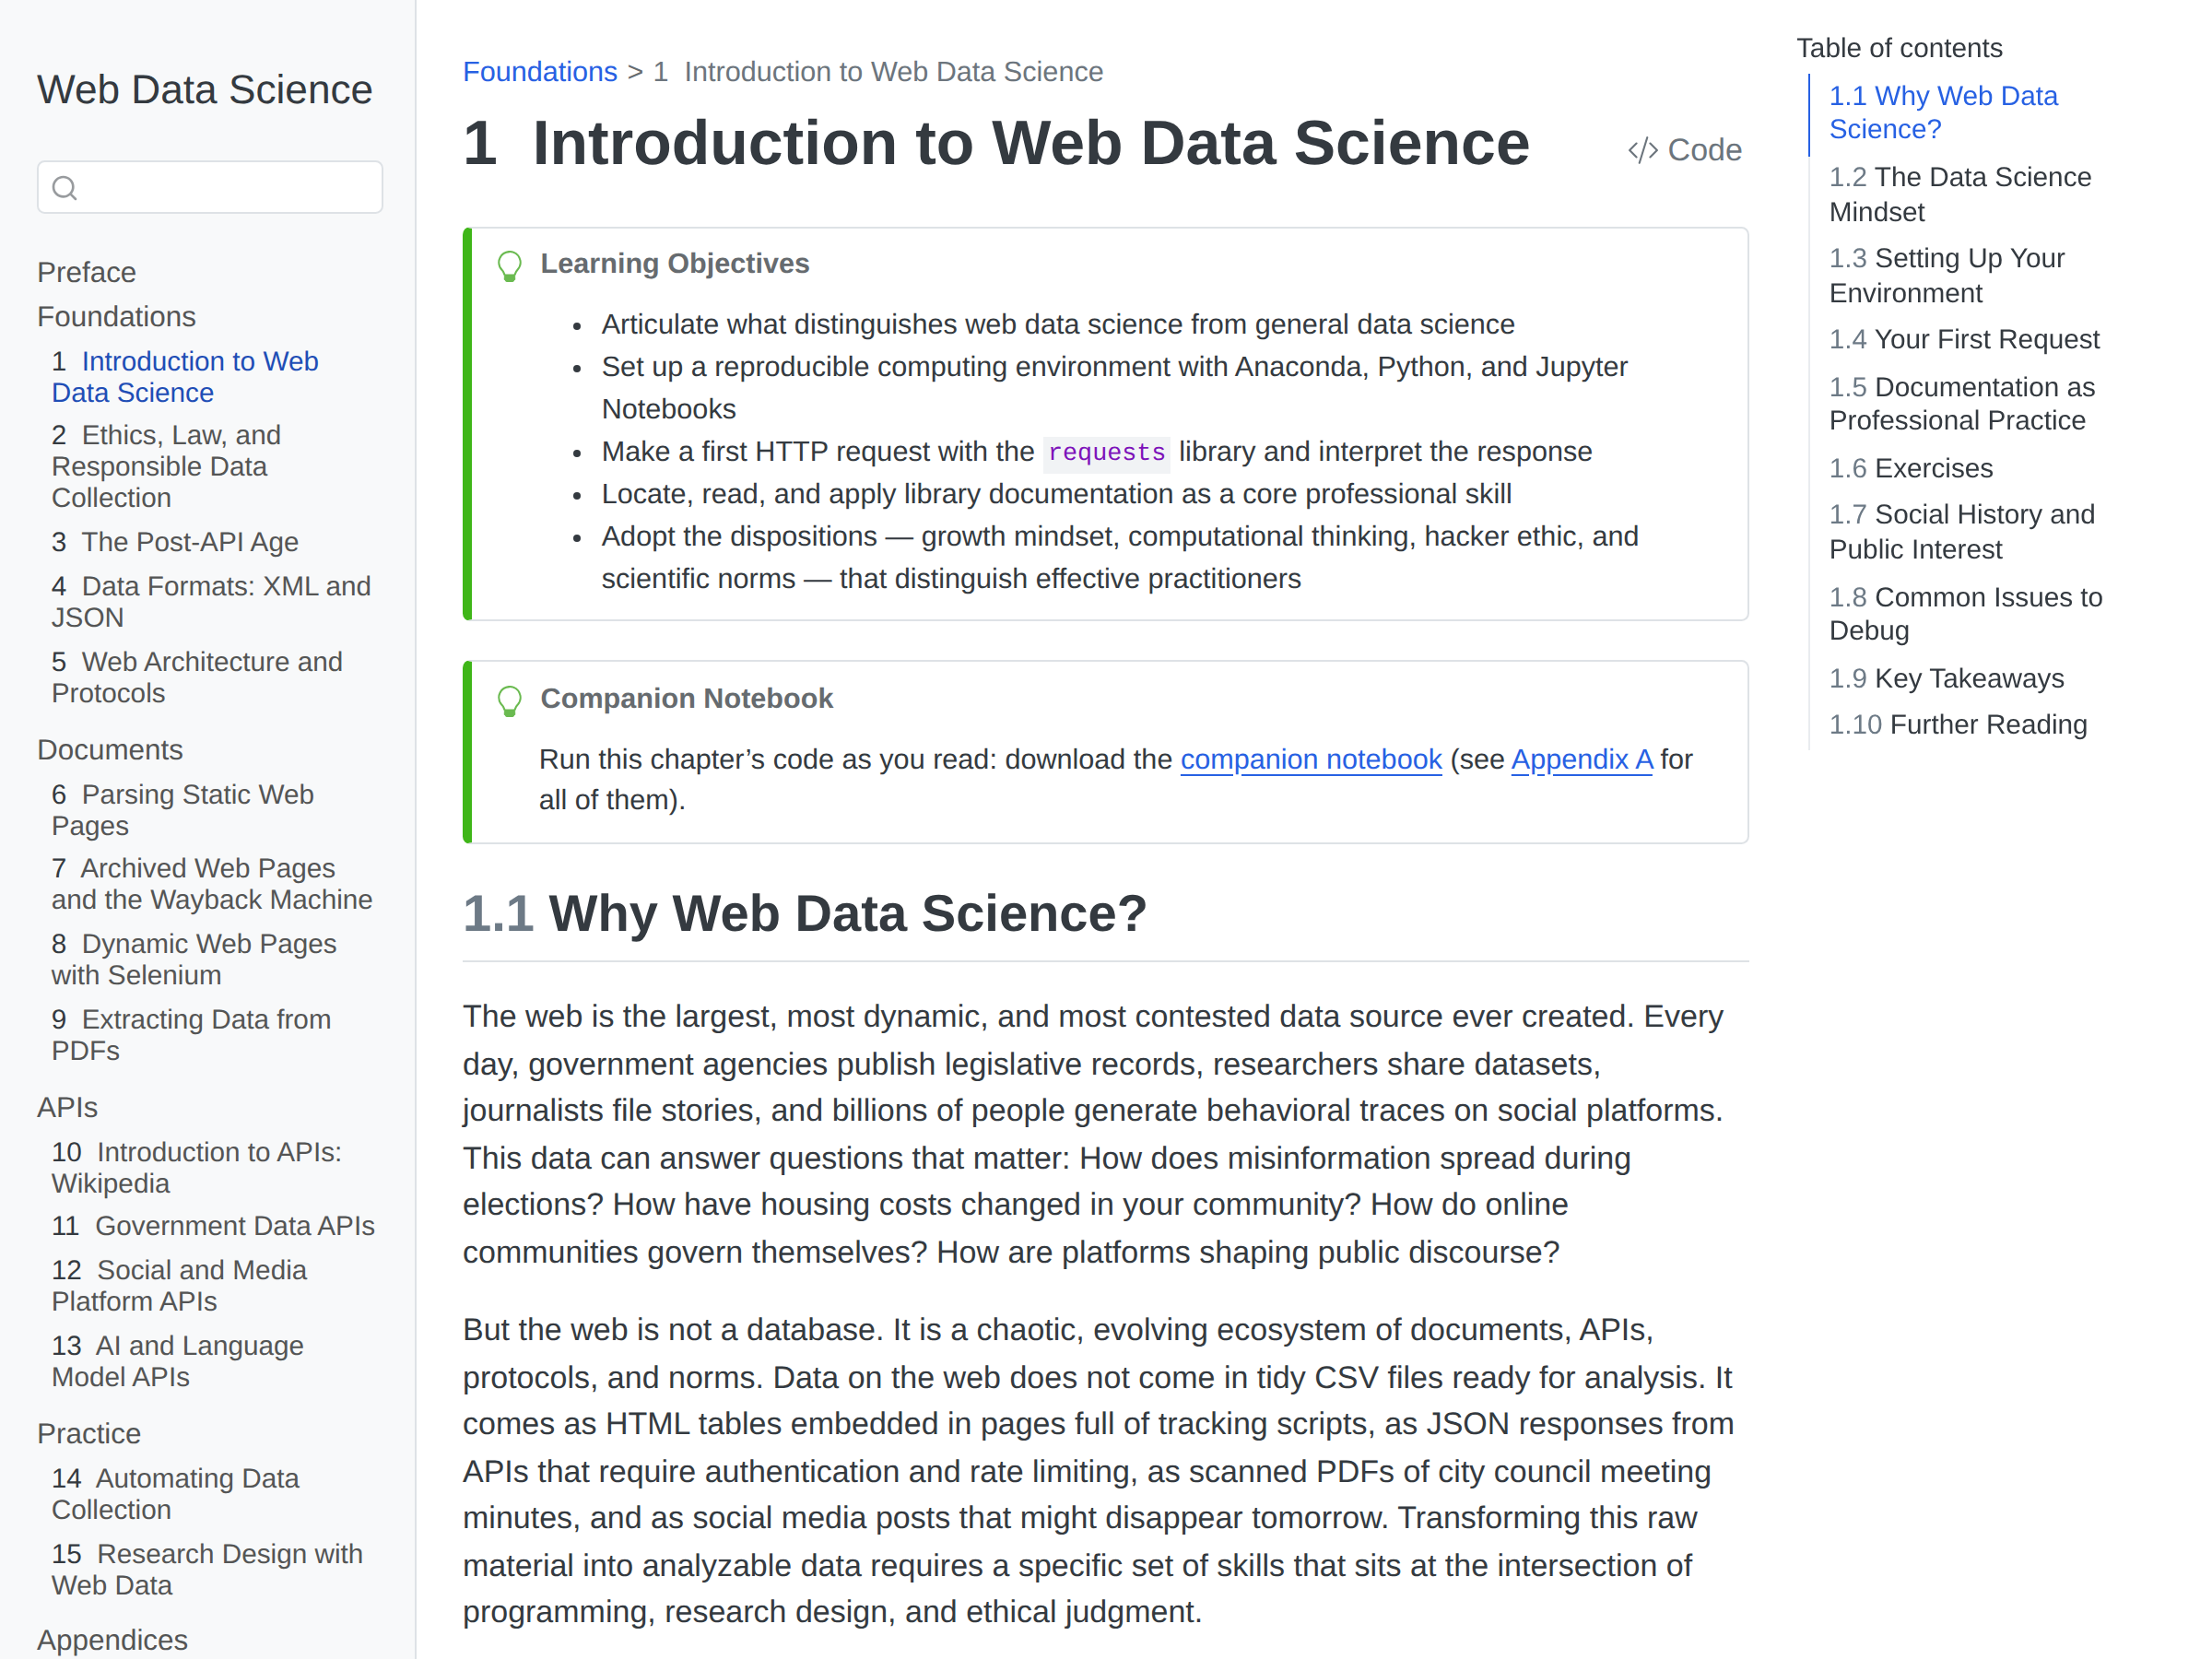
\includegraphics[width=\textwidth]{img/book_website.png}\\
            {\scriptsize The published book --- free, open, and ours to improve.}
        \end{column}
    \end{columns}
\end{frame}

\begin{frame}{How this book was written}
    \begin{columns}[T]
        \begin{column}{0.6\textwidth}
            This book was drafted using large language models $\rightarrow$ there is probably some important stuff that is wrong or confusing
            
            \medskip
            You are going to help me debug, review, edit, verify it
            
            \medskip
            This may not be your first time working with ``AI slop''

            \medskip

            That process is fast and fluent --- and it produces three predictable weaknesses:
            \begin{itemize}\small
                \item \textcolor{tab-red}{\textbf{Confident text that is subtly wrong}} --- a selector that never matched, a parameter that doesn't exist
                \item \textcolor{tab-orange}{\textbf{Explanations from the far side of understanding}} --- correct, but skipping where you actually get stuck
                \item \textcolor{tab-blue}{\textbf{Examples that decay}} --- the web changes underneath the book
            \end{itemize}
        \end{column}
        \begin{column}{0.35\textwidth}
            \begin{alertblock}{Why this matters to you}
                \footnotesize You are meeting this material \textbf{for the first time}. That makes you the best possible reviewer for exactly the failures a fluent draft hides.
                \smallskip

                Your revisions aren't busywork. They're the verification step.
            \end{alertblock}
        \end{column}
    \end{columns}
    \bottomcite{Same standard as the syllabus asks of you: use the tools, verify the output, and disclose the assistance.}
\end{frame}

\begin{frame}{How it's built and published}
    \begin{columns}[T]
        \begin{column}{0.6\textwidth}
            The book is a \textbf{Quarto} project living in a \textbf{GitHub} repository. Nothing about it is a mystery box:

            \medskip

            \begin{enumerate}\small
                \item Each chapter is a plain-text \texttt{.qmd} file --- Markdown with executable code blocks
                \item \texttt{quarto render} turns the \texttt{.qmd} files into the website
                \item GitHub publishes the result at \texttt{cuinfoscience.github.io}
                \item \texttt{references.bib} holds the citations; \texttt{claude.md} documents editorial voice and chapter structure
            \end{enumerate}

            \medskip

            {\footnotesize So ``propose a revision'' concretely means: \textbf{edit a \texttt{.qmd} file} and ask for it to be merged.}
        \end{column}
        \begin{column}{0.35\textwidth}
            \centering
            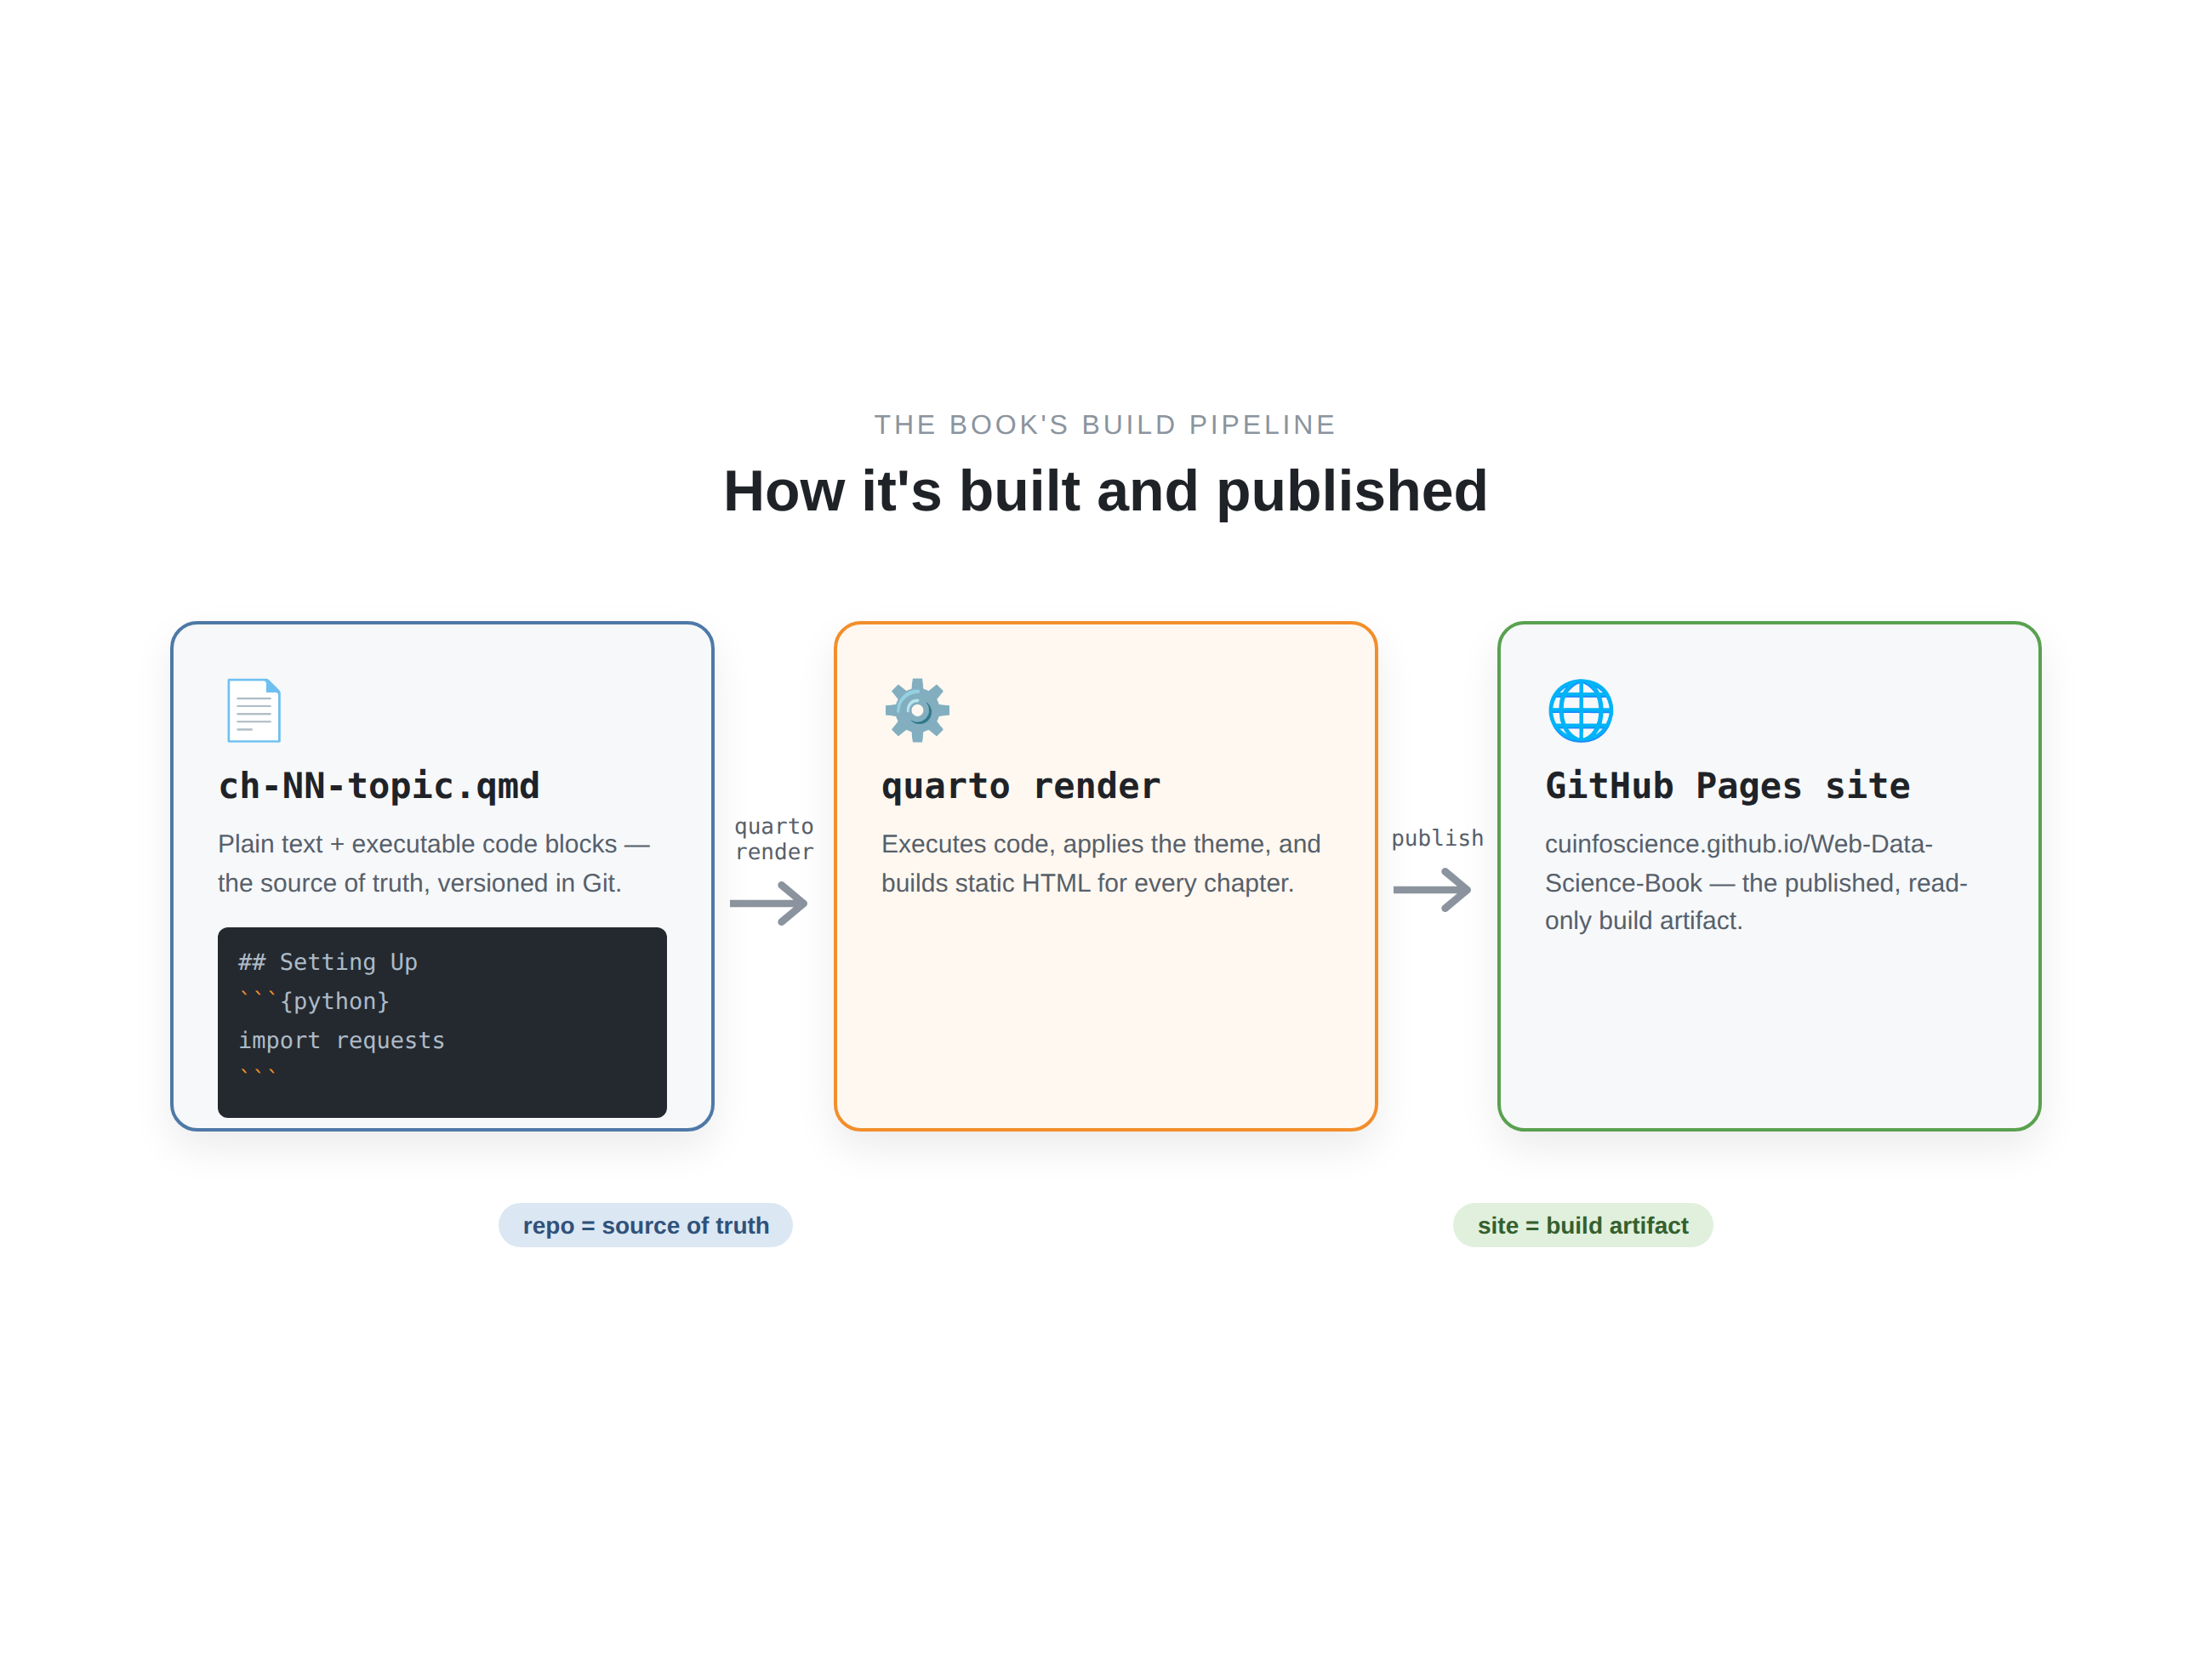
\includegraphics[width=\textwidth]{img/book_pipeline.png}\\
            {\scriptsize Source $\rightarrow$ render $\rightarrow$ published site.}
        \end{column}
    \end{columns}
    \bottomcite{The repository is the source of truth. The website is a build artifact of it.}
\end{frame}

% =========================================================================
\section{Git \& GitHub}
% =========================================================================

\begin{frame}{Git \& GitHub}
    \begin{columns}[T]
        \begin{column}{0.6\textwidth}
            \textbf{Git} records the history of a project --- who changed what, when, and why --- and lets many people work on it without overwriting each other.

            \medskip

            \textbf{GitHub} hosts Git projects online and adds the social layer: proposing, discussing, and reviewing changes.

            \medskip

            Create a free account at \texttt{github.com} with your \textbf{\texttt{colorado.edu}} email to unlock student features. Our textbook lives at:

            \smallskip
            {\footnotesize \texttt{github.com/cuinfoscience/Web-Data-Science-Book}}
        \end{column}
        \begin{column}{0.35\textwidth}
            \centering
            
\includegraphics[width=\textwidth]{img/github_repo.png}\\
            {\scriptsize The book is a living, open repository.}
        \end{column}
    \end{columns}
    \bottomcite{Setup instructions are in \texttt{handouts/setup.md} --- have this working before Monday.}
\end{frame}

\begin{frame}{Four objects you'll use all semester}
    \begin{columns}[T]
        \begin{column}{0.6\textwidth}
            \begin{itemize}
                \item \textcolor{tab-blue}{\textbf{Repository}} --- the project: every file and its full history.
                \smallskip
                \item \textcolor{tab-green}{\textbf{Issue}} --- a written report: ``here is a problem.'' Costs nothing but a browser.
                \smallskip
                \item \textcolor{tab-orange}{\textbf{Pull request}} --- a proposed change: ``here is the fix, side by side with the original.''
                \smallskip
                \item \textcolor{tab-purple}{\textbf{Review}} --- a response to a PR: comment line-by-line, then approve or request changes.
            \end{itemize}
        \end{column}
        \begin{column}{0.35\textwidth}
            \begin{block}{Issue vs.\ pull request}
                \footnotesize An \textbf{issue} says \textit{something is wrong}. A \textbf{pull request} says \textit{here is the correction} --- and shows the exact diff.
                \smallskip

                Issues are cheap and fast; PRs are the real contribution. \textbf{Today you'll file an issue.} From Week 2 on, you'll open pull requests.
            \end{block}
        \end{column}
    \end{columns}
    \bottomcite{This is how essentially all open-source software gets built --- including every library in this course.}
\end{frame}

\begin{frame}{Your Friday workflow}
    \begin{columns}[T]
        \begin{column}{0.6\textwidth}
            From Week 2 onward, every Friday repeats these four steps:
            \begin{enumerate}\small
                \item \textbf{Fork / branch} the book repository
                \item \textbf{Edit} a chapter's \texttt{.qmd} source; commit with a clear message
                \item \textbf{Open a pull request} describing \textit{what} you changed and \textit{why}
                \item \textbf{Review} two classmates' PRs --- kind, specific, and actionable
            \end{enumerate}

            \medskip

            A pull request is a \textbf{proposal}, not an edit. Your change sits next to the original so peers and I can comment line-by-line before anything merges.
        \end{column}
        \begin{column}{0.35\textwidth}
            \centering
            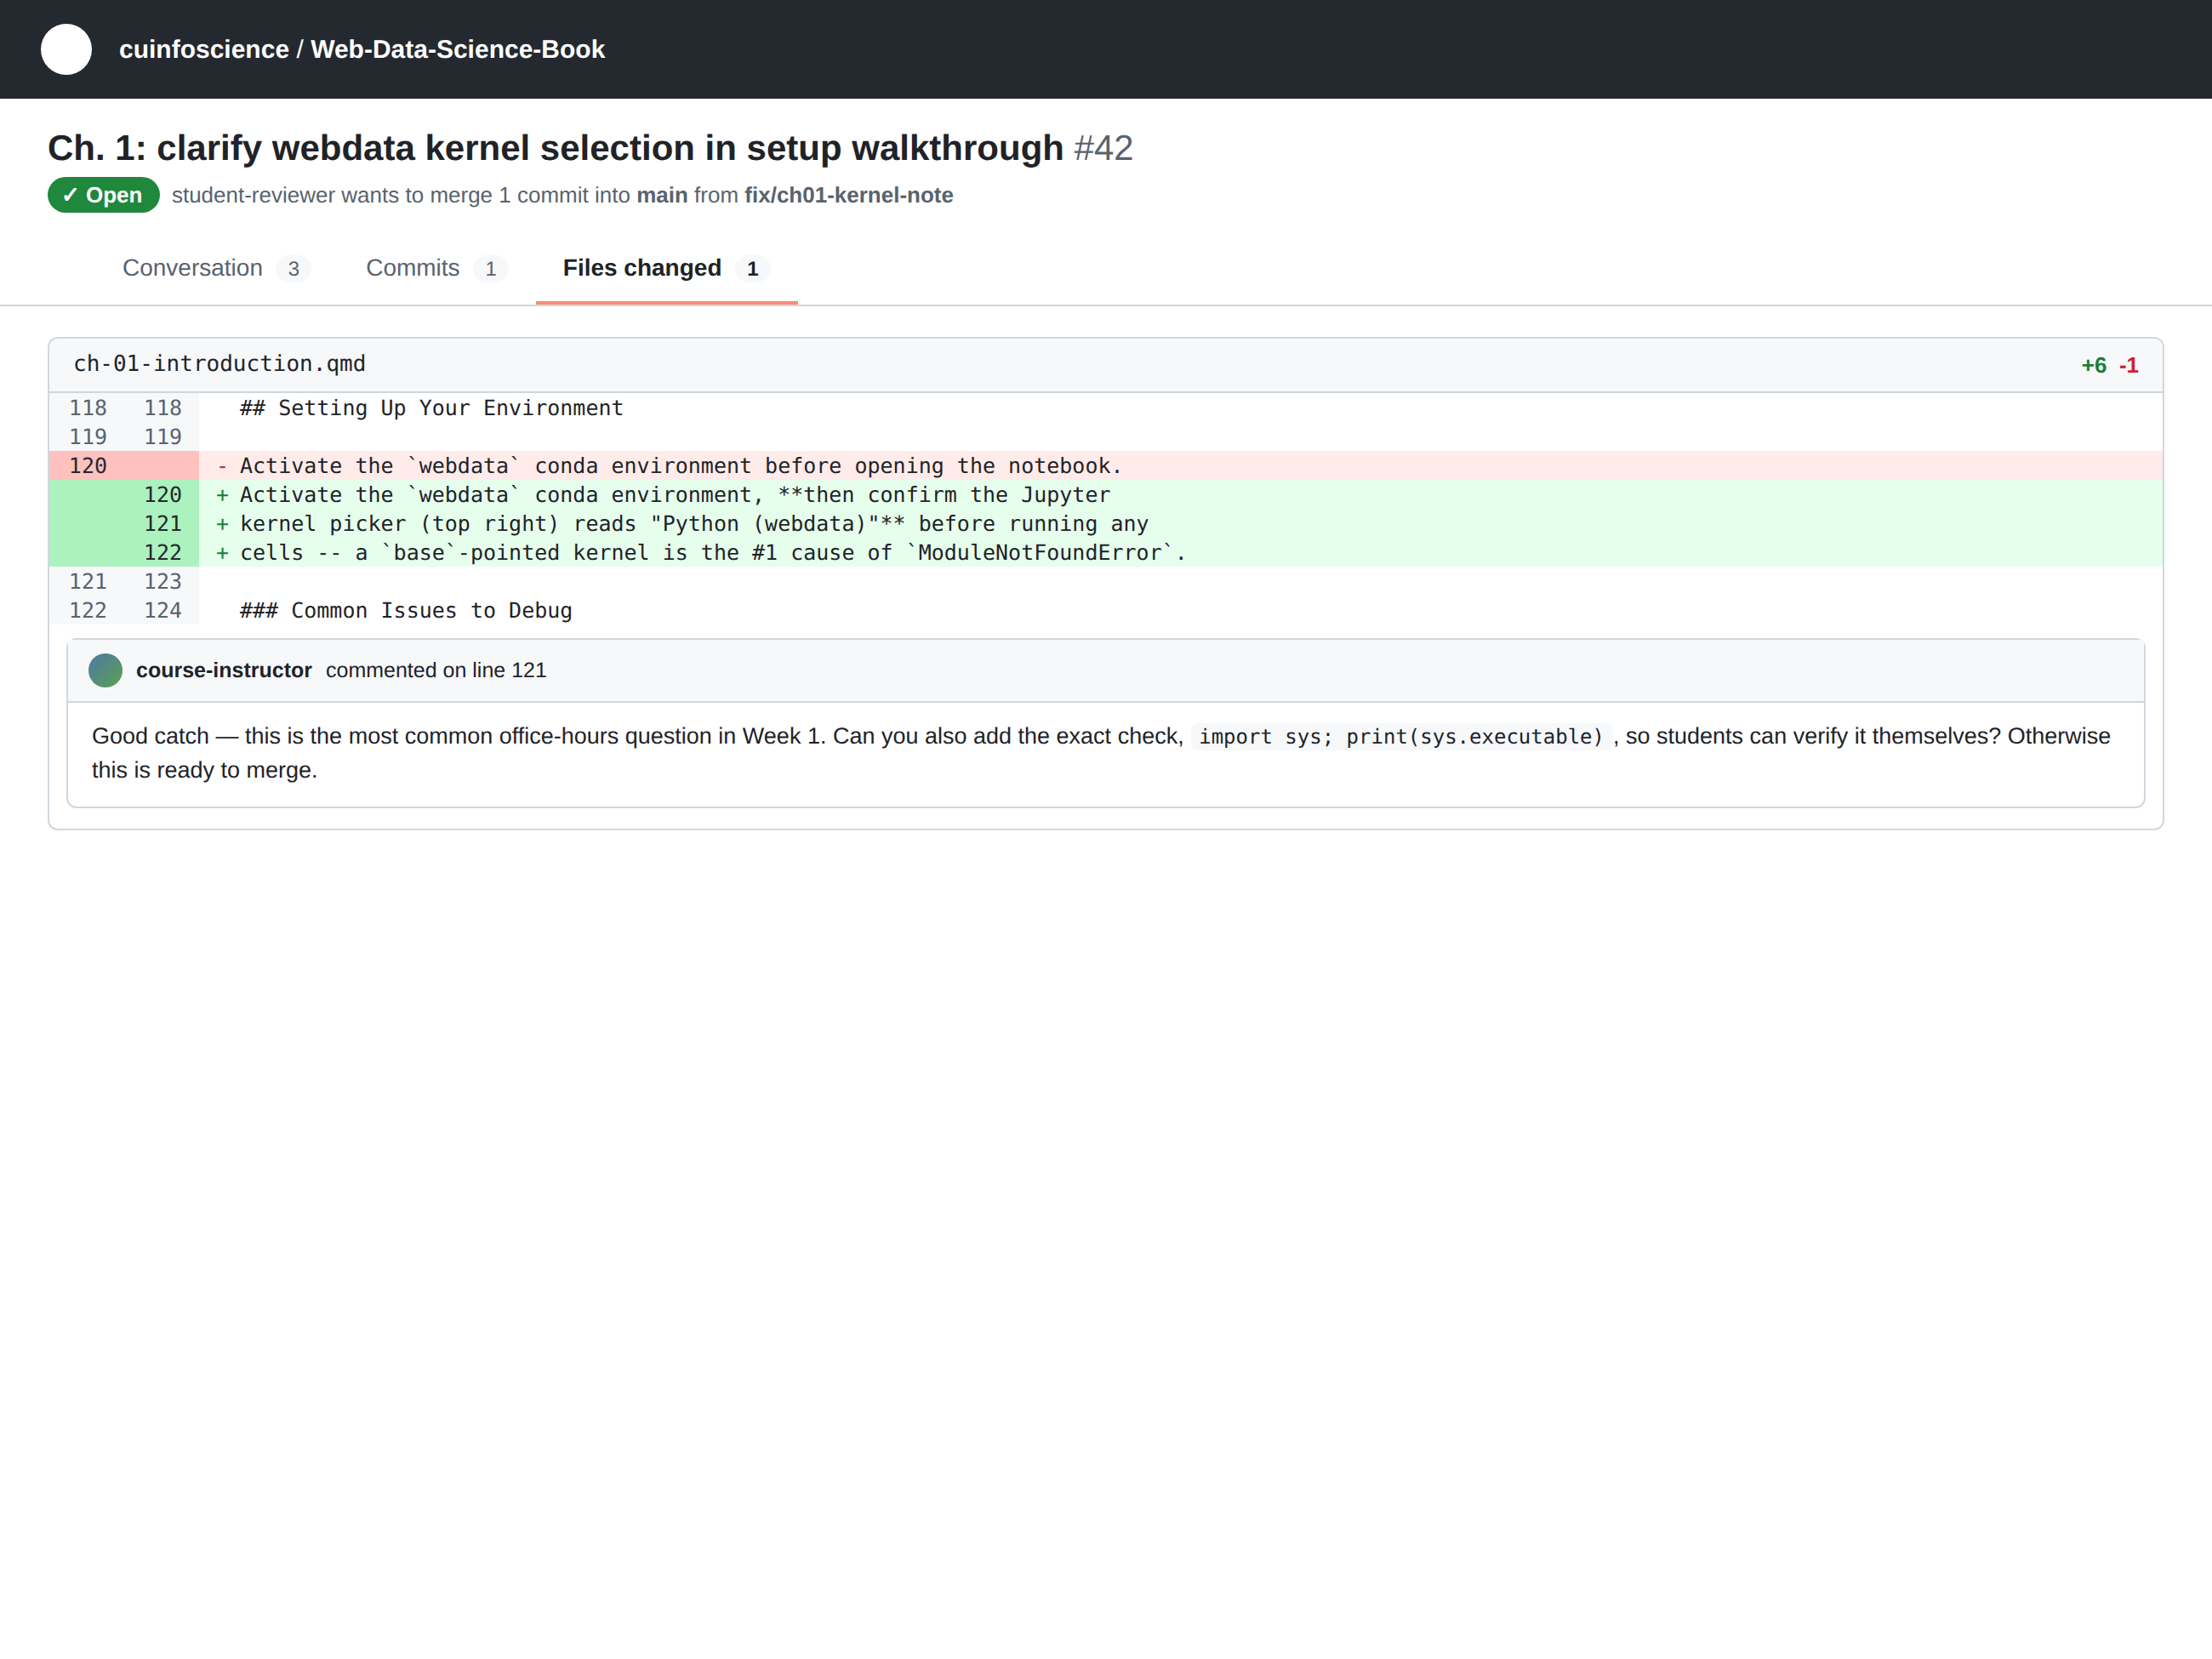
\includegraphics[width=\textwidth]{img/pr_review.png}
        \end{column}
    \end{columns}
    \bottomcite{Contributions \& reviews are the Textbook Revisions grade (30\%). Full workflow walkthrough in Week~2.}
\end{frame}

% =========================================================================
\section{Activity · Propose a revision}
% =========================================================================

\begin{frame}{Today's activity: file your first issue}
    \begin{columns}[T]
        \begin{column}{0.6\textwidth}
            \textbf{Goal:} by the end of class, every one of you has filed one real GitHub issue proposing a change to Chapter~1.

            \bigskip

            \begin{itemize}\small
                \item You need only a \textbf{browser} and a \textbf{GitHub account} --- no Git, no fork, no local copy
                \item Work in pairs; file individually
                \item Read \textbf{Chapter 1} on the published site --- you've just heard the lecture version, so you know what it should have told you
            \end{itemize}

            \medskip

            This is a genuine contribution to a public resource, not a practice exercise.
        \end{column}
        \begin{column}{0.35\textwidth}
            \begin{alertblock}{No account yet?}
                \footnotesize Make one now (2 minutes, \texttt{colorado.edu} email), or pair with someone who has one and draft together.
            \end{alertblock}
            \begin{block}{Timebox}
                \footnotesize \textbf{5} read · \textbf{5} pick \& diagnose · \textbf{8} write \& file · \textbf{5} share out
            \end{block}
        \end{column}
    \end{columns}
\end{frame}

\begin{frame}{Where did the chapter fail you?}
    That question --- not ``what could be added in principle'' --- starts every revision. Sort what you noticed into one of three families:

    \bigskip

    \begin{columns}[T]
        \begin{column}{0.315\textwidth}
            \begin{block}{\textcolor{tab-red}{Broken}}
                \footnotesize It is \textbf{wrong}, or no longer works.
                \smallskip

                \textit{Show:} what you ran, and what happened instead.
            \end{block}
        \end{column}
        \begin{column}{0.315\textwidth}
            \begin{block}{\textcolor{tab-orange}{Unclear}}
                \footnotesize It is right, but you \textbf{couldn't follow it}.
                \smallskip

                \textit{Show:} where you got stuck, and why.
            \end{block}
        \end{column}
        \begin{column}{0.315\textwidth}
            \begin{block}{\textcolor{tab-blue}{Missing}}
                \footnotesize You \textbf{needed something} that wasn't there.
                \smallskip

                \textit{Show:} the gap is real, not merely possible.
            \end{block}
        \end{column}
    \end{columns}

    \bigskip

    \begin{alertblock}{Your inexperience is the qualification}
        \footnotesize Nobody who already knows this material can tell me where a first-time reader falls off. You can --- but only while you're still a first-time reader. That window closes in about a week.
    \end{alertblock}
\end{frame}

\begin{frame}{Seven kinds of revision}
    \begin{table}
    \centering
    \scriptsize
    \begin{tabular}{clll c}
        \toprule
        \textbf{\#} & \textbf{Type} & \textbf{You noticed\ldots} & \textbf{Your contribution includes} & \textbf{Size} \\ \midrule
        1 & \textcolor{tab-red}{\textbf{Code drift}} & An example errors or returns nothing & The error, the fix, what changed upstream & M \\
        2 & \textcolor{tab-red}{\textbf{Stale figure}} & A screenshot doesn't match today's UI & A fresh screenshot, same filename \& crop & S \\
        3 & \textcolor{tab-blue}{\textbf{Common issue}} & An error not in ``Common Issues to Debug'' & Symptom $\rightarrow$ cause $\rightarrow$ fix, in the list's format & S \\
        4 & \textcolor{tab-blue}{\textbf{Missing figure}} & You sketched it yourself to understand it & The figure, a caption, and alt text & M \\
        5 & \textcolor{tab-blue}{\textbf{Reading}} & A claim with no source behind it & The citation in \texttt{references.bib} + why it belongs & S \\
        6 & \textcolor{tab-orange}{\textbf{Exercise}} & An exercise is ambiguous or unverifiable & Expected output, a rubric, or a starter cell & M \\
        7 & \textcolor{tab-orange}{\textbf{Explanation}} & You reread a passage three times & The rewrite + what confused you the first time & M \\
        \bottomrule
    \end{tabular}
    \end{table}

    \smallskip

    \begin{columns}[T]
        \begin{column}{0.6\textwidth}
            {\footnotesize \textbf{Type 3 is the easiest high-value contribution in the book} --- it converts your lost debugging time into somebody else's saved time.}
        \end{column}
        \begin{column}{0.35\textwidth}
            {\footnotesize \textbf{Size} = review effort. \textbf{S}: a few lines. \textbf{M}: a paragraph or code block. Bigger than M? File an issue first.}
        \end{column}
    \end{columns}
    \bottomcite{The full framework, with worked examples of each type: \texttt{handouts/revision-framework.md}}
\end{frame}

\begin{frame}{How issues \& pull requests are graded}
    \begin{columns}[T]
        \begin{column}{0.6\textwidth}
            Weekly, out of \textbf{10 points} --- the Textbook Revisions grade (30\%).
            \medskip
            \begin{table}
            \centering
            \footnotesize
            \begin{tabular}{llc}
                \toprule
                \textbf{Criterion} & \textbf{Full marks} & \textbf{Pts} \\ \midrule
                \textbf{Located} & Chapter, section \& file named & 2 \\
                \textbf{Evidenced} & I can reproduce what you hit & 3 \\
                \textbf{Actionable} & A concrete change, scoped to one thing & 3 \\
                \textbf{Reviews} & Two peer reviews, specific, with a verdict & 2 \\ \midrule
                & \textbf{Total} & \textbf{10} \\
                \bottomrule
            \end{tabular}
            \end{table}
            \medskip
            {\footnotesize Most weeks, most people land at \textbf{7--9}. A 10 means someone could act on your proposal without asking a single follow-up question.}
        \end{column}
        \begin{column}{0.35\textwidth}
            \begin{alertblock}{Merged is not the bar}
                \footnotesize You're graded on the \textbf{proposal and the review}, not on whether I merge it. A well-evidenced PR I decline for editorial reasons earns full credit. A merged one-character typo fix does not.
            \end{alertblock}
            \begin{block}{Little or no credit}
                \footnotesize
                \begin{itemize}\footnotesize
                    \item Bulk typo PRs
                    \item ``This is confusing'' with no location or proposal
                    \item Duplicates --- check open issues first, then \textit{review} theirs
                    \item Undisclosed AI text you didn't verify
                \end{itemize}
            \end{block}
        \end{column}
    \end{columns}
\end{frame}

\begin{frame}{Writing it: the skeleton}
    \begin{columns}[T]
        \begin{column}{0.6\textwidth}
            Every issue and every PR description uses the same five fields:

            \medskip

            \begin{itemize}\small
                \item \textbf{Title} --- \texttt{<type>: <specific thing> in Ch. N}
                \item \textbf{Location} --- chapter, section, and the \texttt{.qmd} file
                \item \textbf{Problem} --- what you did, expected, and got. Paste the code and output.
                \item \textbf{Why} --- who this affects, in one sentence
                \item \textbf{Proposal} --- the concrete change you'd make
            \end{itemize}

            \medskip

            {\footnotesize Can't fill in \textbf{Location} and \textbf{Problem} with specifics? You don't have a revision yet --- you have a hunch. Go back and reproduce it.}
        \end{column}
        \begin{column}{0.35\textwidth}
            \begin{block}{Worked example}
                \footnotesize
                \textbf{Title:} Common issue: kernel/environment mismatch in Ch.~1
                \smallskip

                \textbf{Location:} \texttt{ch-01-introduction.qmd}, ``Setting Up Your Environment''
                \smallskip

                \textbf{Problem:} Installed \texttt{requests} in \texttt{webdata}, but the notebook raised \texttt{ModuleNotFoundError}. The kernel was pointing at base.
                \smallskip

                \textbf{Why:} Likely to hit anyone using conda environments --- cost me 20 minutes.
                \smallskip

                \textbf{Proposal:} Add to ``Common Issues'': check \texttt{sys.executable} in the notebook.
            \end{block}
        \end{column}
    \end{columns}
    \bottomcite{One change per issue or PR. Three fixes in one PR is three reviews wearing one coat.}
\end{frame}

\begin{frame}{Your turn}
    \begin{columns}[T]
        \begin{column}{0.6\textwidth}
            \begin{enumerate}
                \item \textbf{Read} Chapter 1 on the published site --- skim for the parts you'd have needed today \hfill {\scriptsize(5 min)}
                \item \textbf{Pick one} problem. Name its family and its type from the table \hfill {\scriptsize(5 min)}
                \item \textbf{Check} the repo's open issues --- if yours exists, comment on it instead \hfill {\scriptsize(1 min)}
                \item \textbf{Write and file} it using the five-field skeleton \hfill {\scriptsize(8 min)}
                \item \textbf{Share out} --- a few of you read yours aloud \hfill {\scriptsize(5 min)}
            \end{enumerate}
        \end{column}
        \begin{column}{0.35\textwidth}
            \centering
            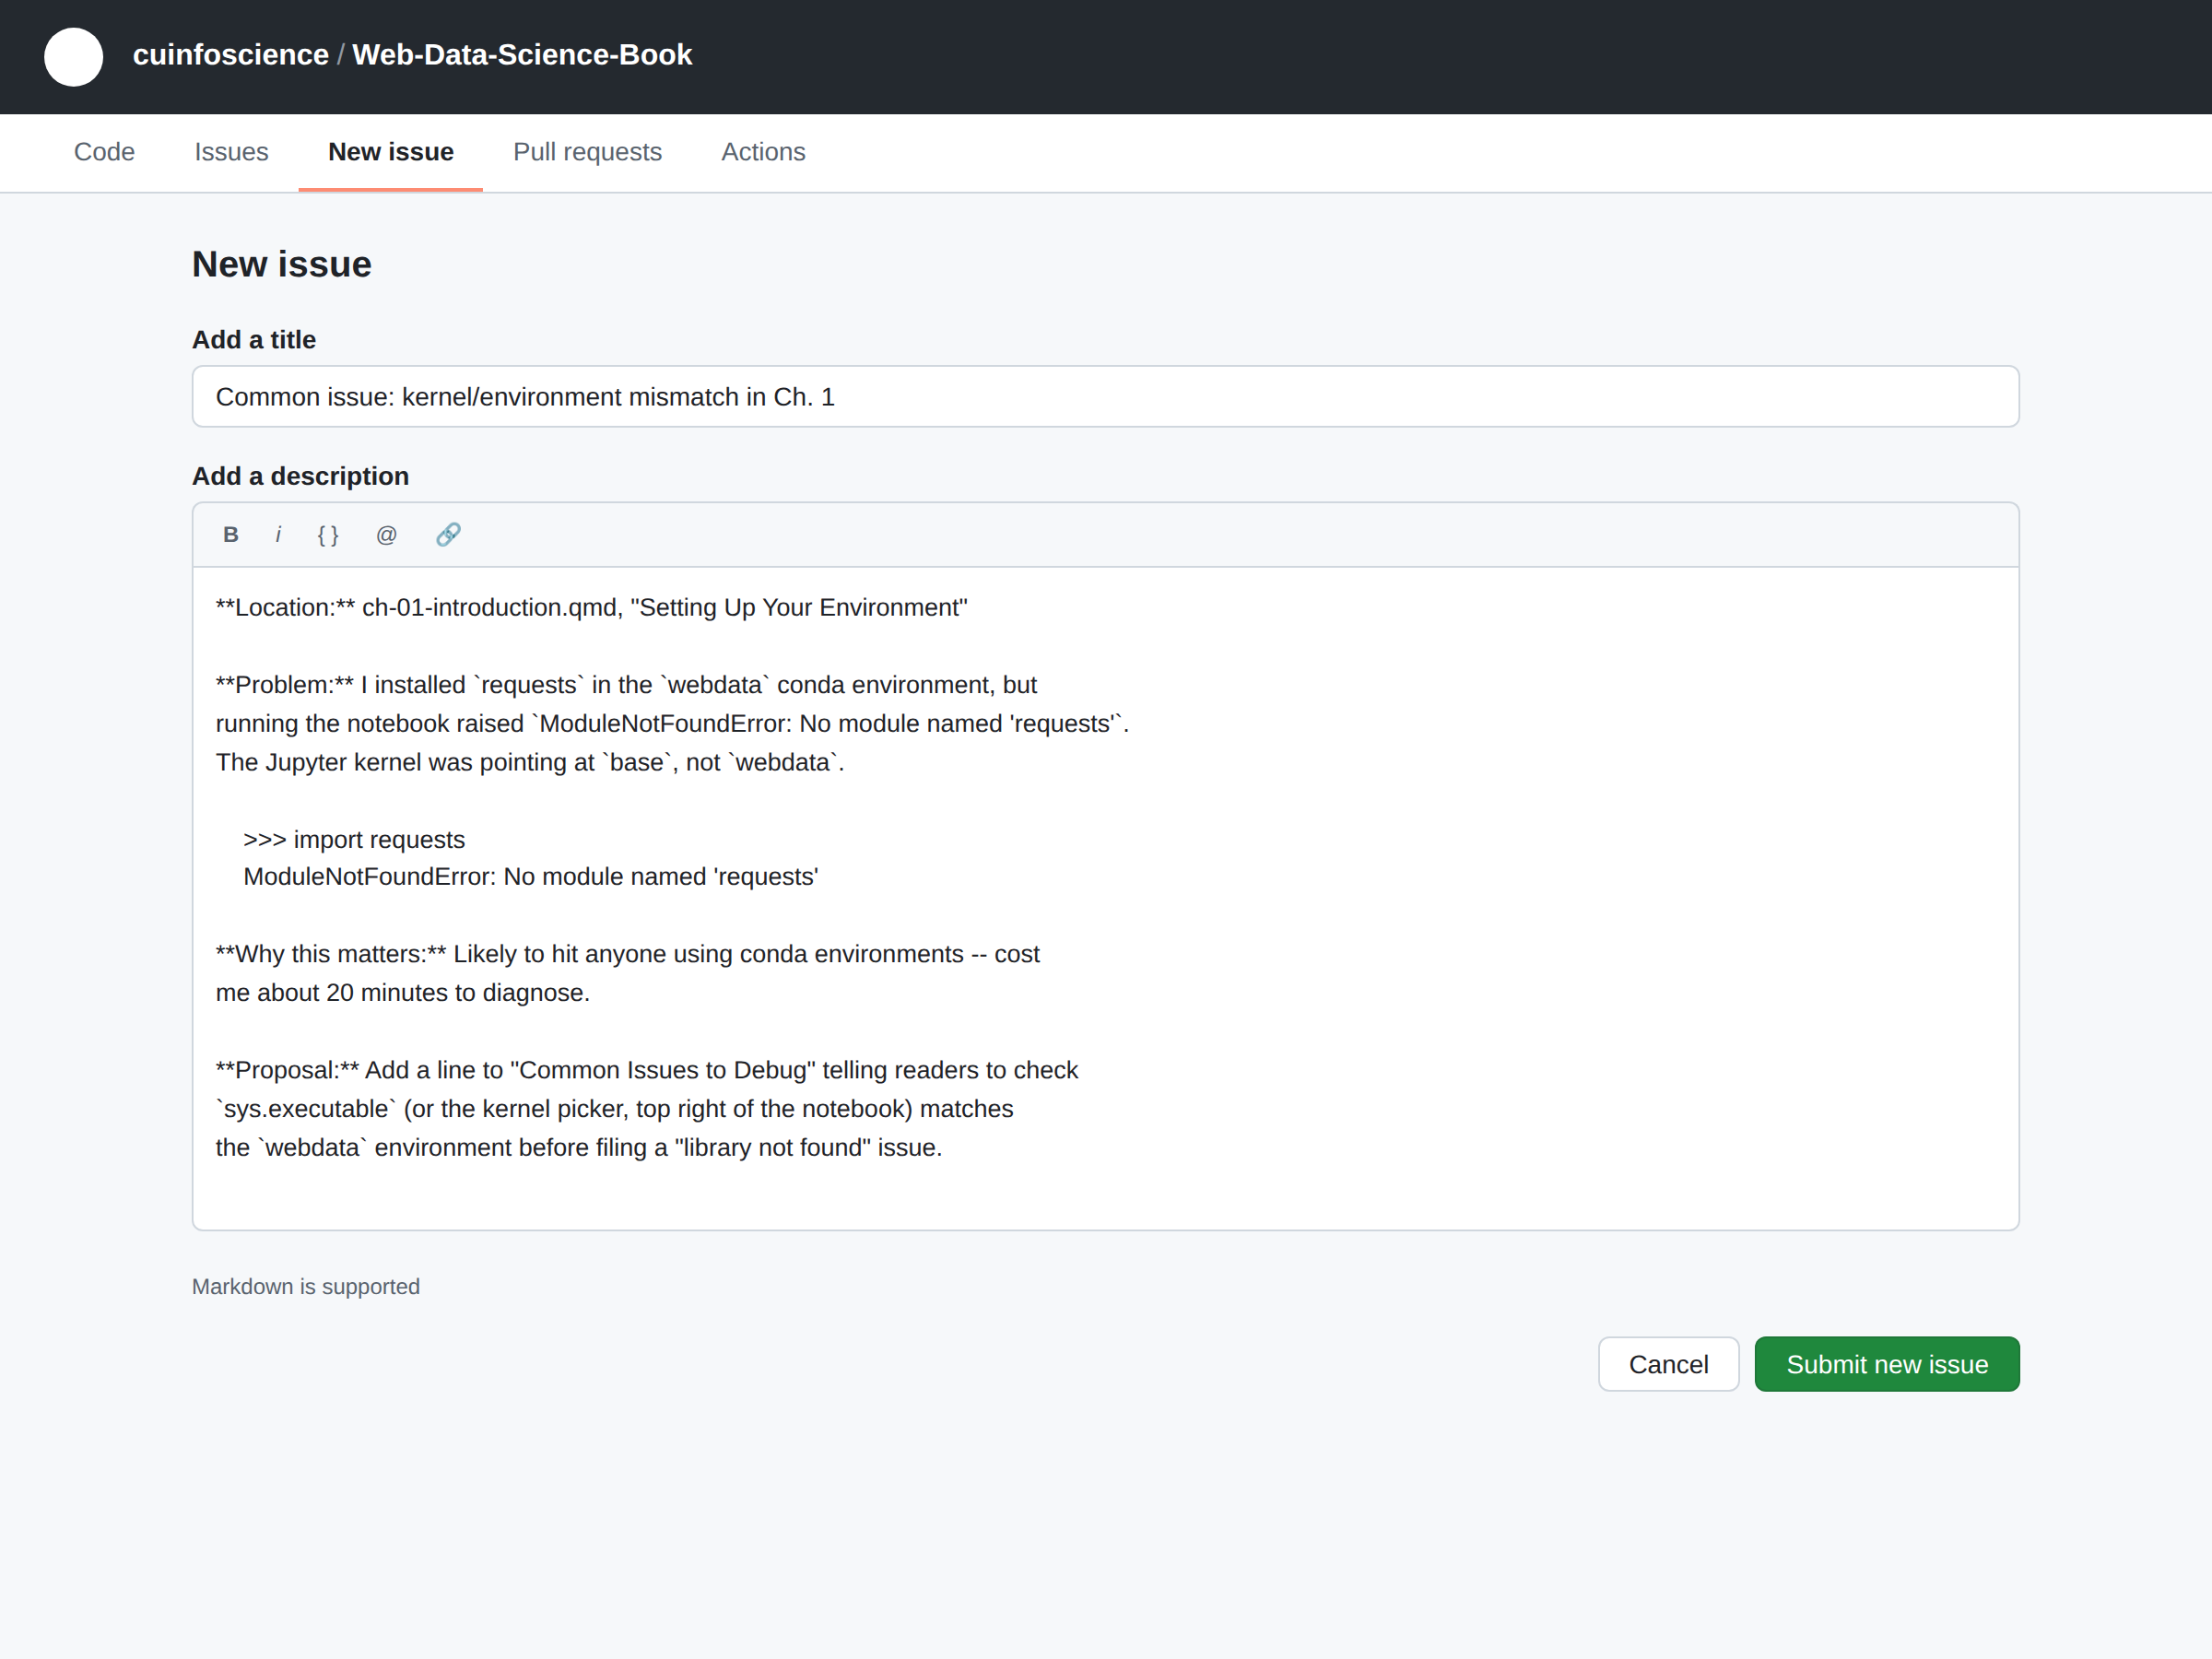
\includegraphics[width=\textwidth]{img/issue_form.png}\\
            {\scriptsize \texttt{Issues} $\rightarrow$ \texttt{New issue} --- that's the whole mechanism.}
            \medskip

            \begin{alertblock}{Next week}
                \footnotesize Your issue becomes your \textbf{first pull request} --- you'll fix the thing you found.
            \end{alertblock}
        \end{column}
    \end{columns}
    \bottomcite{Stuck choosing? ``The chapter never told me X, and I needed X'' is always a legitimate issue.}
\end{frame}

% =========================================================================
\section{Before you go}
% =========================================================================

\begin{frame}{Before Monday}
    \begin{columns}[T]
        \begin{column}{0.6\textwidth}
            Work through \texttt{handouts/setup.md} --- about 45 minutes:
            \begin{enumerate}
                \item \textcolor{tab-blue}{\textbf{Python, via Anaconda}} --- plus a \texttt{webdata} environment and the core libraries
                \item \textcolor{tab-green}{\textbf{Git}} --- installed and configured with your name and email
                \item \textcolor{tab-orange}{\textbf{A free GitHub account}} --- with your \texttt{colorado.edu} address
            \end{enumerate}
            \medskip
            The handout ends with a two-cell check: retrieve a page, then pull Wikipedia pageviews into a DataFrame. \textbf{If it runs, you're ready.}
        \end{column}
        \begin{column}{0.35\textwidth}
            \begin{alertblock}{Don't suffer in silence}
                \footnotesize Email me \textbf{before Monday} if setup fails --- arriving with a broken environment costs you the lab.
                \smallskip

                Can't access a laptop or install software? Contact me \textbf{immediately} so we can arrange an accommodation.
            \end{alertblock}
        \end{column}
    \end{columns}
    \bottomcite{Also read Textbook Ch.~2 (Ethics, law \& responsible collection) before Monday.}
\end{frame}

\begin{frame}[standout]
    The web is not a database.\\
    It's a chaotic, evolving ecosystem of documents, APIs, and norms.\\[1em]
    {\large Your first challenge isn't modeling ---\\ it's getting the data at all.}
\end{frame}

% =========================================================================
\begin{frame}{Key takeaways}
    \begin{enumerate}
        \item Web data science is \textbf{retrieve $\rightarrow$ parse $\rightarrow$ analyze} --- and the hard part is getting the data at all.
        \item Every week has a rhythm: \textbf{Monday} concept, \textbf{Wednesday} notebook lab, \textbf{Friday} textbook-revision pull requests.
        \item The textbook is \textbf{open, Quarto-built, and AI-drafted under human review} --- which is exactly why your first-time-reader perspective is valuable.
        \item Revisions sort into \textbf{Broken / Unclear / Missing} and seven concrete types. Graded on \textbf{location, evidence, actionability, and reviews} --- not on whether I merge them.
        \item Your grade is what you build: Labs 30\%, Revisions 30\%, Final Project 40\% --- \textbf{no exams}.
    \end{enumerate}
    \medskip
    \centering\small Next week: \textbf{Ethics, law \& responsible collection} --- \texttt{robots.txt}, Terms of Service, and how to collect data without doing harm.
    \bottomcite{Reading: Textbook Ch.~1--2. Related: \textcite{salganik2018bit}; \textcite{wilson2017good}.}
\end{frame}

\end{document}
